\documentclass[a4paper,10pt]{article}
\usepackage[utf8]{inputenc}
\usepackage[english]{babel}
\usepackage{graphicx}
\usepackage{amsmath}
\usepackage{acronym}
\usepackage{titling}
\usepackage{import}
\usepackage{listings}
\usepackage{hyperref}
\usepackage{float}	
\usepackage[hang,small,sc]{caption}
\usepackage{subcaption}
\usepackage{tikz}



% ------------------------------------------------------------
% Acronyms
% ------------------------------------------------------------
\acrodef{FTP}{File Transfer Protocol}
\acrodef{CBR}{Constant bitrate}
\acrodef{TCP}{Transmission Control Protocol}
\acrodef{UDP}{User Datagram Protocol}

\newcommand{\HRule}{\rule[0em]{\linewidth}{0.2mm}}

\setlength{\droptitle}{-2.0cm}
\newcommand{\subtitle}[1]{%
  \posttitle{%
    \par\end{center}
    \begin{center}\large#1\end{center}
    \vskip0.5em}%
}

%------------------------------------------------------------------------------
%   TitlePage
%------------------------------------------------------------------------------
\title{Network Simulation with \texttt{ns/2}: report}
\subtitle{G0Q43A - Computer Networks}

\preauthor{\vskip 1.0em %
\HRule%
\vskip 2.0em%
\begin{center}
\large \lineskip 0.5em%
\begin{tabular}[t]{c}}
\postauthor{\end{tabular}\par\end{center} %
%    \begin{flushleft}\large{\hskip0.6em r0382389}\end{flushleft}
    \vskip1.5em%
}

\predate{\vspace{-1.6em}%
\begin{flushright} \begin{tabular}[t]{c}}

\postdate{\end{tabular}\par\end{flushright}}

\author{Martinus Wilhelmus Tegelaers  \and Thomas Vochten}
\date{\today}


%opening

\begin{document}
	\maketitle

	%abstract
	\begin{abstract}
This report describes the use of the \verb|ns/2| network event simulator to simulate the behaviour of simple network topologies.
Two topology situations are considered. For the first situation, the focus lies on an \ac{FTP} application competing for bandwidth with a \ac{CBR} application. 
In the second situation, we investigate the evolution of the congestion window size during the execution of the \ac{TCP} algorithm in detail; an \ac{FTP} application is running continuously while a web user on the same LAN as the \ac{FTP} application generates short intense bursts of traffic. We also compare congestion window size behaviour between
the Tahoe implementation of \ac{TCP} and the Reno implementation of \ac{TCP}.
\end{abstract}
	%exercises
	\section{Exercise 1: Bandwidth restrictions on KotNet}
	\begin{enumerate}
		\item \textbf{First, leave out the connection of the uploader. Plot the throughput of the main \ac{FTP} connection and discuss the download behaviour of a KotNet/Telenet modem with bandwidth caps. How do bandwidth limitations affect the download connection?}
		
		The throughput of the \ac{TCP} destination node is plotted in figure \ref . The default \ac{TCP} Tahoe implementation was used. The granularity of the throughput was set at 0.1s. 
		The \ac{TCP} connection is started at 1.0s. The throughput raises exponentially until the 4.0Mb cap of the network is reached. This can be attributed to the slow start feature of \ac{TCP}. At this point the throughput stays around 4.0 Mb until the connection is closed at 9.9s. 
		The negative bumps in the throughput are the result of the congestion window resetting to one. In figure \ref the congestion window is plotted. The bumps in the throughput are at the same time as when the congestion window resets. These resets take place when time-outs occur, or the receiver indicates that it has reached its limit. 
		
		When the congestion window is small, the number of packages sent is small, but due to the exponential growth, the effect is fairly limited. 		

		The small positve bumps above the 4.0 Mb are caused by rounding errors. These would be smaller with a smaller granularity. 
		
		\item \textbf{What happens if you now enable both upload and download activities? Plot and compare the throughput of both streams. Do you spot any problems? If so, explain.}
		
		The throughputs of the receiving \ac{TCP} node and the receiving \ac{CBR} node are plotted in figure \ref. The \ac{TCP} throughput starts out in the same manner as in fig. \ref, again the throughput is capped at 4.0Mbs, due to the modem link. At 3.0s the \ac{CBR} application starts, and immediately the throughput of the \ac{TCP} connection drops significantly. It is crippled until the \ac{CBR} connection is stopped at 6.8s. At this point the normal slow start pushes the throughput back to 4.0Mbs, until the \ac{TCP} connection is stopped at 9.9s. 
		The decrease in the throughput of the \ac{TCP} connection is due to the upload channel getting congested by the \ac{CBR} application. The underlying \ac{UDP} connection does no congestion control, thus it floods the upload buffers of the modem. This causes packets to be dropped, which in turn causes the congestion window to reset often, thus leading to a far lower throughput. 
		The \ac{CBR} does no congestion control, as mentioned earlier, thus it will just flood the modem, and fill it till the capped 256.0Kbs. 
		
		\item \textbf{Consider now that the model is able to guarantee a certain amount of upload bandwidth to every application, which performance do you expect for both applications (\ac{FTP} and \ac{CBR})?}
		
			The \ac{FTP} application will perform better if the guaranteed upload bandwidth is big enough to send the acknowledgements without dropping them. Then a similar download performance will be observed as in fig \ref. 
			The smaller the guaranteed upload bandwidth, the more likely it is packages will be dropped, and performance will drop.
			The \ac{CBR} might lose some of its performance, as a part of the total bandwidth will be allocated to the \ac{FTP} application. However since it is not a hard cap, only a guarantee, this would only cause performs drops when the \ac{FTP} application, or other processes, would be actively using their guaranteed bandwidth. 
		
		\item \textbf{What would be the result if bandwidth was even more restricted? For example, up to September 2010, KotNet limitations were 512Kbps for downstream traffic and 100Kbps for upstream traffic.}
		
		  	In figure \ref the results of the an even more restricted bandwidth are plotted. The graph has a similar curvature as fig. \ref. However the \ac{TCP} connection now has a throughput of zero at times. This is due to the higher number of congestion window resets.
		  	Thus the results would be that performance of the \ac{FTP} application would be even more crippled with a more restricted bandwidth.
		
		\item \textbf{Configure the upload connection with a fixed \texttt{rate\_} of 30k. Explain the simulated result (no plot required). What would be your (extra) solution(s) to improve the download experience on shared LANs behind capped Internet connections? How could you practically realise this?}
		
		By setting the rate of the \ac{CBR} application to 30k, the upload speed of the \ac{CBR} application is restricted to only 32Kbs.  The \ac{CBR} application is thus no longer capable of congesting the upload channel of the modem. This in turn, will benefit the \ac{FTP} applications' performance, since its packages will no longer be lost. 
		This effect can be observed in fig. \ref. The \ac{TCP} throughput is at the maximum 4.0Mbs, the \ac{CBR} connection is limited at only 32Kbs. 
		
		It would be possible to switch from \ac{TCP} Tahoe to \ac{TCP} Reno, which causes smaller drops than \ac{TCP} Tahoe. Another improvement could be to use delayed acknowledgements. 		
		
		\item \textbf{Suppose we have in the future a KotNet/Telenet cable subscription that has 10 times more capacity: i.e a connection that has a downstream capacity of 40Mbps with an upstream capacity of 2Mbps.}
		
			\begin{enumerate}
			  	\item \textbf{What performance can you expect if there are 10 users behind this connection and all performing the same activities as in this exercise? Why? What performance can you expect if there are only 5 users using the network? Why?}
			  	
			  	The performance of the \ac{TCP} would be bad, due to all the additional \ac{CBR} applications. As mentioned earlier, \ac{CBR} application have no form of congestion control and will flood the buffers of the modem again. The increased buffer size will not be enough to hold all upload packages, and will in turn drop certain packages.  The acknowledgements of the \ac{TCP} connection will be dropped, and thus performance will drop. 
			  	
			  	If there were only five users, the buffers might not get filled completely, which would improve the performance of the \ac{TCP} connection. This would lead to less packages of the \ac{TCP} connection to be dropped, and thus increasing throughput. 
			  	
				\item \textbf{Does the performance differ if 10 users perform the same activities but at random times? Are there some users who suffer from the network activities caused by other users? Why?}
				
				The worst case scenario would be that all users would upload at the same time, thus flooding the upload buffers, and creating a congestion. If the users start at random times, the upload activities would be scattered over a greater interval, thus most likely decreasing the amount of congestion. This would have a positive effect on the performance. 
				The \ac{FTP} downloaders would still be affected by the \ac{CBR} uploaders. Especially when multiple \ac{CBR} uploaders are uploading at the same time, performance would plummet. 
			\end{enumerate}
	\end{enumerate}
	\section{Exercise 2: Tahoe and Reno versus bursty web traffic}
\begin{enumerate}
 \item \textbf{Investigate the throughput of the main FTP application. Can you indicate the effects the
 individual bursts of web traffic have on its total throughput? Why do these ffects not immediately
 become visible when each burst starts (i.e. at 5, 10 , or resp. 15 seconds)?} \\
 
 Figure \ref{fig:ex2throughput} shows the throughput of the main FTP application. We can see that the throughput rises
 rapidly at the start before hitting the bandwidth limit within the first 700 milliseconds. Thereafter, it remains at $1.25$
 megabytes/s. When the first burst begins at 5 seconds, we see a drop to 800 kilobytes/s as the first TCP connection for the web user
 starts, but the throughput can still climb to one megabytes/s. It is only after 700 milliseconds that the throughput
 decreases dramatically. When the burst starts, new connections between the web user and the web server are opened within
 about 0.05 milliseconds. These connections first go through the slow start phase of TCP, which means it takes some time
 before each connection attains a throughput that could affect existing connections. Soon, the 10 megabytes/s bandwidth
 limit cannot support high throughputs for each active connection, which means the main FTP connection experiences packet loss. This triggers
 congestion avoidance for the main FTP application and it sets its congestion window to 1 kilobyte, after which it
 must go through slow start again. \\
 
 After about 8 seconds, the main FTP application has to contend with increasingly fewer connections from the web user,
 which allows the throughput to climb steadily. A new burst starts at 10 seconds, and this time the effects manifest
 themselves after 300 milliseconds. This is again explained by connections being opened one after another and
 each connection gradually increasing its throughput. \\
 
 Right before the third burst, the FTP application cuts its throughput because of congestion. The throughput is allowed
 to climb until 15.7 seconds, when the new burst first has an impact. From 17 seconds on, more and more web connections
 finish their work, allowing the FTP application to steadily increase its throughput to the highest allowed bandwidth
 across the network.
 
 \begin{figure}[h]
 \label{fig:ex2throughput}
  \centering
    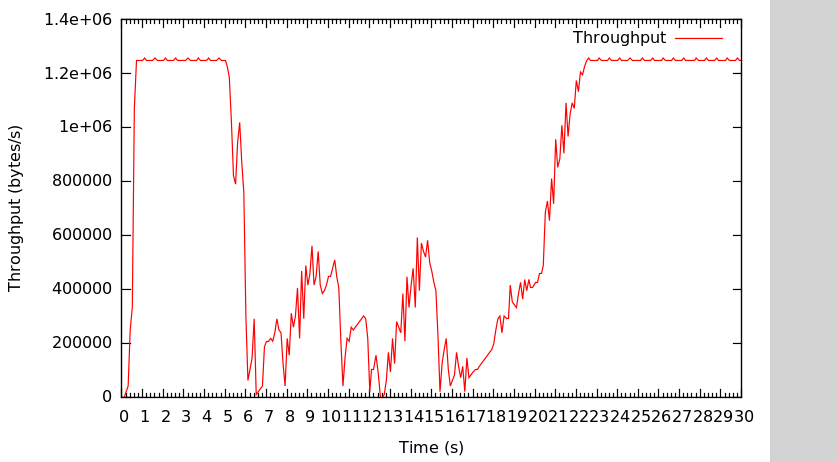
\includegraphics[scale=0.5]{ex2throughput.png}
  \caption{The throughput of the continuously running FTP application. Ticks are drawn every 200 milliseconds.}
 \end{figure}
 
 \item \textbf{Plot the congestion window size and
 slow start thresholds in another graph. Can you identify
 the different phases of the TCP algorithm? When is the
 slow start threshold recalculated and how?} \\
 
 Figure \ref{fig:ex2congestionwindow} shows the congestion window sizes and the slow start thresholds for the main
 FTP application. To start off, the threshold is set to 80 packets and the congestion window to 1 packet. Each time
 the sender receives an acknowledgement, the congestion window is set to $min(2 \cdot window size, threshold)$.
 This is the slow start phase. Once the threshold has been reached, the window size increases linearly. This is
 the additive increase phase. At about 5.76 seconds, the FTP application experiences a packet loss, which causes
 the window size to drop to one packet. The slow start threshold is set to $max(2, \frac{threshold}{2})$, which in
 this case is 40. After that, the slow start phase begins again.
 
 \begin{figure}[h]
 \label{fig:ex2congestionwindow}
  \centering
    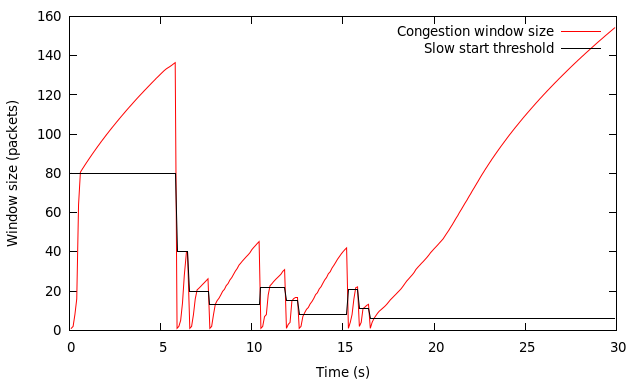
\includegraphics[scale=0.5]{ex2congestionwindow.png}
  \caption{The congestion window sizes and slow start thresholds for the main FTP application running TCP Tahoe.}
 \end{figure}
 
 \item \textbf{Discuss the AIMD principle of TCP. Take one 'sawtooth' pattern in the graph and indicate a few
 reasonable values for the congestion window on the graph. What is the first interval the TCP congestion avoidance
 algorithm is active?} \\
 
 AIMD stands for Additive Increase Multiplicative Decrease. It is the idea where one wants to increase the congestion window
 size by one each round-trip time and, when necessary, decrease the window size multiplicatively. In TCP Tahoe, this
 multiplicative decrease is implemented by cutting the window size to one packet if packet loss occurs. TCP diverges
 from the principle by the use of slow start, where the window size increases exponentially (by always doubling the
 window size) until a pre-defined threshold is reached. After that, it goes back to additive increase. \\
 
 When one plots the behaviour exhibited by a connection that abides by the AIMD principle, it produces a sawtooth pattern.
 There are periods where the congestion window size increases, overshoots the optimal window size, decreases, falls
 below the optimal window size and then increases again. The effect is that the congestion window size converges
 to the optimal value. Looking at the moment where the first burst begins at 5 seconds in \ref{fig:ex2congestionwindow},
 there is a first drop to a size of one packet. After that, slow start is activated again and the window size increases
 rapidly to 40 packets, after which congestion manifests itself again. The next slow start increases until a size of 20,
 after which additive increase continues for about 600 milliseconds when there is packet loss again. After this drop,
 the intensity of the current burst decreases. This behaviour suggests that a congestion window size of 20 would have been
 a reasonable value during this burst.
 
 \item \textbf{Change the TCP implementation of the main FTP application into Reno. Plot the congestion window
 and slow start thresholds. Do you spot the differences with the default TCP Tahoe implementation? Why does the
 window sometimes still drop to zero or one?} \\
 
 Figure \ref{ex2congestionwindowreno} shows the behaviour for the TCP Reno implementation. Looking at the congestion drop
 that occurs at approximately 10.6 seconds, it can be seen that both the congestion window size and the slow start threshold
 are set to $max(2, \frac{threshold}{2})$
 
 \begin{figure}[h]
 \label{fig:ex2congestionwindowreno}
  \centering
    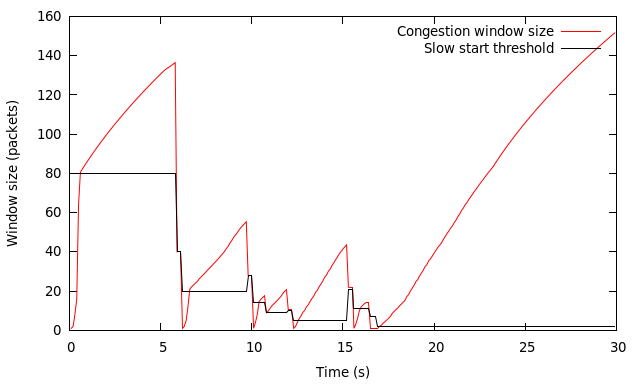
\includegraphics[scale=0.5]{ex2congestionwindowreno.png}
  \caption{The congestion window sizes and slow start thresholds for the main FTP application running TCP Reno.}
 \end{figure}
 
 
\end{enumerate}
\end{document}